\begin{figure}[bt!]
  \begin{center}
    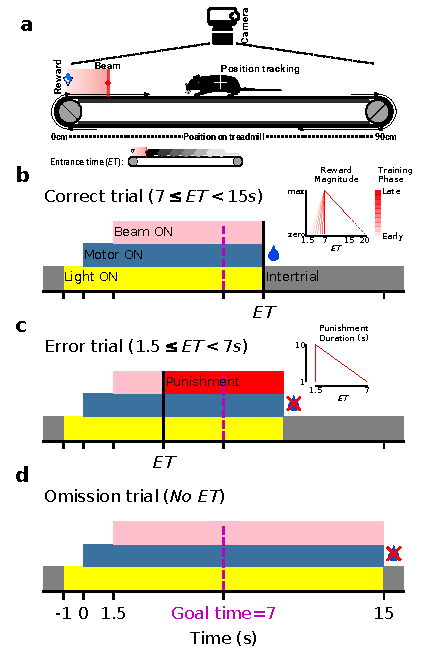
\includegraphics[scale=1]{ch-methods/figures/TaskRulesFULL.pdf}
    \caption[Treadmill Task]
        {\textbf{Treadmill task and trial types.}
        \textbf{a)}
        Rats were enclosed on a powered treadmill. 
        The infrared beam marked the reward area (red shaded area).
        During each trial, the belt pushed the animals away from the reward area and the first infrared beam interruption defined the \gls{et}.
        During trials and intertrials, the animal's position was tracked via a ceiling-mounted video camera.
        \textbf{b)}
        Schematic description of a rewarded correct trial.
            \textit{Inset}: the magnitude of the delivered reward dropped linearly as \gls{et} increased (maximum reward at \acrlong{gt}).
            In early stages of training, smaller rewards were delivered for trials with $ET<7$~s.
            However, the smallest \gls{et} value that triggered reward delivery was progressively raised during learning.
        \textbf{c)}
        Schematic description of an error trial.
        Early \glspl{et} triggered an extra-running penalty and an audio noise.
            \textit{Inset}: the duration of the penalty period was 10~s for the shortest \glspl{et} and fell linearly to 1~s for \glspl{et} approaching 7~s.
        \textbf{d)}
        Schematic description of an omission trial (no beam crossing between 1.5~s and 15~s).
        \textbf{b-d)}
        Note that \glspl{et} started to be detected 1.5~s after the motor start. 
    }
    \label{fig:methods:taskRules}
  \end{center}
\end{figure}